%%%%%%%%%%%%%%%%%%%%%%%%%%%%%%%%%%%%%%%%%%%%%%%%%%%%%%%%%%%%%%%
\PassOptionsToPackage{subsection=false}{beamerouterthememiniframes} % delete subsection line
\documentclass{beamer}
\usepackage{tikz}
\usepackage{array}
\usepackage{url}
\usepackage{amsmath, amsthm, amsfonts, amssymb}
\usepackage{booktabs}
\usepackage{enumerate}
\usepackage[shortlabels]{enumitem}
\usepackage{pifont}
\usepackage{framed}
\usepackage{textcomp}
\usepackage{xeCJK}
\usepackage{caption}
\usepackage{subcaption}
\usepackage{fontspec}
\usepackage[natural, svgnames]{xcolor}
\usepackage{natbib}
\bibliographystyle{econ}
\usepackage{hyperref}
\hypersetup{
    colorlinks,
    citecolor=myblue,
    linkcolor=myblue,
    urlcolor=myred
}

%%%%%%%%%%%%%%%%%%%%%%%%%%%%%%%%%%%%%%%%%%%%%%%%%%%%%%%%%%%%%%%
% beamer theme setting
\usetheme{Szeged}
\usecolortheme{rose}
\usefonttheme{serif}

%%%%%%%%%%%%%%%%%%%%%%%%%%%%%%%%%%%%%%%%%%%%%%%%%%%%%%%%%%%%%%%
% Unable the control buttons at bottom
\setbeamertemplate{navigation symbols}{}

%%%%%%%%%%%%%%%%%%%%%%%%%%%%%%%%%%%%%%%%%%%%%%%%%%%%%%%%%%%%%%%
% Color definition
\definecolor{myred}{RGB}{192,46,46}
\definecolor{myblue}{RGB}{7,75,164}
\definecolor{mygreen}{rgb}{0.11,0.7,0.02}

%%%%%%%%%%%%%%%%%%%%%%%%%%%%%%%%%%%%%%%%%%%%%%%%%%%%%%%%%%%%%%%
% Modify the footer display
\newcommand{\shortauthor}{\textcolor{myblue}{Yu-Chieh Kuo}}
\setbeamertemplate{footline}
{%
  \begin{beamercolorbox}[colsep=1.5pt]
      {upper separation line foot}
  \end{beamercolorbox}
  \hbox{%
      \begin{beamercolorbox}[wd=0.333333\paperwidth, ht=4ex, 
          dp=2.3ex, leftskip=.3cm plus1fill, rightskip=.3cm]
          {title in head/foot}%
          \usebeamerfont{title in head/foot}
          \parbox{.28\paperwidth}{\raggedright\inserttitle}
    \end{beamercolorbox}%
    \begin{beamercolorbox}[wd=0.333333\paperwidth, ht=4ex, 
        dp=2ex, center]{title in head/foot}%
      \usebeamerfont{author in head/foot}
      \insertframenumber/\inserttotalframenumber
    \end{beamercolorbox}%
    \begin{beamercolorbox}[wd=0.333333\paperwidth, ht=4ex,
        dp=2ex, leftskip=.3cm, rightskip=.3cm plus1fil]
        {title in head/foot}%
        \usebeamerfont{title in head/foot}
        \parbox{.28\paperwidth}{\raggedleft\shortauthor}
    \end{beamercolorbox}}
  \begin{beamercolorbox}[colsep=1.5pt]
      {lower separation line foot}
  \end{beamercolorbox}
}

% Modify section and subsection's entry
\setbeamertemplate{section in toc}{
  {\color{myblue}\inserttocsectionnumber.}~\inserttocsection}
\setbeamertemplate{subsection in toc}{
\hspace{1.2em}{\color{myblue}$\triangleright$}~\inserttocsubsection\par}

% Modify itemize's entry and position
\setlist[itemize]{label=\textcolor{myblue}{$\triangleright$}}
\setlength{\leftmargini}{0pt}

% Modify beamer color setting
\setbeamercolor{block title}{use=structure, fg=white, bg=myblue!90!white}
\setbeamercolor{block body}{use=structure, fg=black, bg=myblue!20!white}
\setbeamercolor{block title alerted}{use=structure, fg=white, bg=myred!90!white}
\setbeamercolor{block body alerted}{use=structure, fg=black, bg=myred!20!white}
\setbeamercolor{frametitle}{fg=myblue}
\setbeamercolor{separation line}{bg=myblue}
\setbeamercolor{section in head/foot}{fg=myblue}
\setbeamercolor{subsectiopn in head/foot}{fg=myblue}
\setbeamercolor{section in toc}{fg=myblue}
\setbeamercolor{subsection in toc}{fg=myblue}
\setbeamercolor*{title}{fg=myblue}
\setlist[description]{format=\textcolor{myblue}}

% Modify margin setting
\justifying
\setbeamersize{text margin left=1.8em,text margin right=1.8em}
\setlength{\parindent}{2em}

\addtobeamertemplate{frametitle}{\setlength{\parindent}{0em}}{}
\addtobeamertemplate{block begin}{\setlength{\parindent}{0em}}{\setlength{\parindent}{2em}}
\addtobeamertemplate{block example begin}{\setlength{\parindent}{0em}}{\setlength{\parindent}{2em}}
\settowidth{\leftmargini}{\usebeamertemplate{itemize item}}
%\addtolength{\leftmargini}{\labelsep}

% Set Chinese font and English font
\setCJKmainfont{思源宋體 TW}
\setmainfont{Philosopher}
%\setmainfont{Apple Chancery}
\newfontfamily\chancery{Apple Chancery}
\setbeamerfont{title}{size=\huge, series=\bfseries}
\DeclareTextFontCommand{\textch}{\chancery}

%%%%%%%%%%%%%%%%%%%%%%%%%%%%%%%%%%%%%%%%%%%%%%%%%%%%%%%%%%%%%%%
% array enviornment shortcut

\newcolumntype{R}{>{\displaystyle}r}
\newcolumntype{C}{>{\displaystyle}c}
\newcolumntype{L}{>{\displaystyle}l}

%%%%%%%%%%%%%%%%%%%%%%%%%%%%%%%%%%%%%%%%%%%%%%%%%%%%%%%%%%%%%%%
% Title page information

\title{
    The Beneficial Effects of Ad Blockers
}  
\author{Yu-Chieh Kuo\inst{1}} 
\date{\today} 

\institute[NTU]
{
    \inst{1}
    Department of Information Management,
    National Taiwan University
}

%%%%%%%%%%%%%%%%%%%%%%%%%%%%%%%%%%%%%%%%%%%%%%%%%%%%%%%%%%%%%%%
% Display the toc page in the beginning of every section
% but hide all subsections for personaly needs

\AtBeginSection[]
{
    \begin{frame}[noframenumbering]
      \frametitle{}
      \tableofcontents[currentsection, hideallsubsections]
    \end{frame}
}

%%%%%%%%%%%%%%%%%%%%%%%%%%%%%%%%%%%%%%%%%%%%%%%%%%%%%%%%%%%%%%%
% Topic-based command setting

\newcommand{\hl}[1]{\textcolor{myblue}{#1}}
\newcommand{\ban}{\textch{\textcolor{myblue}{Ban}}}
\newcommand{\al}{\textch{\textcolor{myblue}{Allow}}}
\newcommand{\fee}{\textch{\textcolor{myblue}{Fee}}}
\newcommand{\ad}{\textch{\textcolor{myblue}{Ads}}}
\newcommand{\aof}{\textch{\textcolor{myblue}{Ads or Fee}}}
\newcommand{\wl}{\textch{\textcolor{myblue}{White-List}}}
\newcommand{\ab}{\text{ad-block users }}
\newcommand{\nab}{\text{non-ad-block users }}
\newcommand{\cc}{\text{content creators }}

%%%%%%%%%%%%%%%%%%%%%%%%%%%%%%%%%%%%%%%%%%%%%%%%%%%%%%%%%%%%%%%

% This command is used to ignore frames without specifying their label at "current" to
% accelerate the compiling process. If you want to compile a complete slide,
% comment it and compile "twice" by xeLaTeX.
%\includeonlyframes{current}


%\noindent
\begin{document}

\begin{frame}
\titlepage
\end{frame} 
\begin{frame}[label=current]
    \frametitle{Background}
    \begin{itemize}
        \item
        Online advertising is the lifeline of many internat content platforms,
        whose revenue highly depends on ad.
        \begin{itemize}
            \item
                \$59.6 B in the US in 2015.
            \item
                Almost half of it accounted for by Big Techs.
        \end{itemize}
        \item However, people do not want to see ads when surfing the web.
        \begin{itemize}
            \item The ad blocking usage is ascending over years, especially
                on the mobile devices and softwares.
        \end{itemize}
    \item Online platforms lost huge revenues due to the ad blocker.
\end{itemize}
\end{frame}

\begin{frame}
    \frametitle{Question}
    \begin{itemize}
        \item It comes to some question:
        \begin{itemize}
            \item Why do not the companies and platforms forbid the use
            of ad-blocking software even it is easy to erect a block wall?
            \item What is the idea behind the platforms which allow the ad blocker?
            \item What is the optimal response of platforms under different 
            scenarios?
        \end{itemize}
    \end{itemize}
\end{frame}

\begin{frame}
    \frametitle{Ingredient}
    \begin{itemize}
        \item What may be the important element to the analysis?
    \end{itemize}

    \begin{description}
        \item[Competition:] 74\% of ad-block users say they leave websites
            when faced with an ad-block wall. This may be the key point
            why platforms do not adopt ad-block walls.
        \item[Ad. Intensity:] 77\% of ad-block users say they are willing 
            to view some ad and are not totally against ads.
        \item[Ad. Sensitivity:] People are heterogeneous of ad sensitivity
            across sites and devices.
    \end{description}
\end{frame}

\begin{frame}[label=current]
    \frametitle{Literature Reviews}
    \framesubtitle{}
    \begin{itemize}
        \item Many researchers discuss about advertising and marketing avoidance, for example,
            \citet{Clancey} and \citet{Speck} emphasized it before 2000, which may be 
            regarded as the very previous literatures in this issue.
        \item In addition, lots of literatures, such as \citet{Johnson} and \citet{Anderson}
            analyze the model of marketing targets and ad usages on marketing.
        \item However, most prior work focused on traditional media, such as TV,
            rather than web media, where web ads, ad blockers, and anti-ad-block technology
            develop rapidly. 
            \begin{itemize}
                \item Of course, researchers nowaday notice this field and some of them are
                    interested in
                    it. A similar work is \citet{Aseri}.
            \end{itemize}
    \end{itemize}
\end{frame}

\begin{frame}
    \frametitle{Agenda}
    \tableofcontents[hideallsubsections]
\end{frame} 

\section{Model Setting} 
\begin{frame}
\frametitle{Platforms} 
\begin{itemize}
    \item There are two platforms, platform 1 and platform 2,
        competing over a set of users. Platforms profit from ads.
    \item Each platform can choose one of 
        three different strategies: \ban, \al, or \fee. 
    \item The platform's decision variables for each strategy are
        \textcolor{myblue}{ad intensity $a_i\geq0$}
        and \textcolor{myblue}{subscription fee $p_i\geq 0$}.
    \item Their profits are
        \[
            \begin{array}{L}
                \Pi_i^\ban = \text{(\# users picking platform $i$)}\cdot a_i \\[3mm]
                \Pi_i^\al = \text{(\# users picking platform $i$ and seeing ads)}
                \cdot a_i \\[3mm]
                \Pi_i^\fee = \text{(\# users picking platform $i$)}\cdot p_i
            \end{array}
        \]
\end{itemize}
\end{frame}

\begin{frame}
    \frametitle{Users}
    \begin{itemize}
        \item We model users using a \hl{Hotelling line}.
            \begin{itemize}
                \item Assume that the two platforms are located on the endpoints
                    of the interval $[0,1]$.
                \item Users are distributed uniformly from $[0,1]$. 
                    For users at position $x$, they obtain $1-x$ 
                    if they pick platform 1 and $x$ if they pick platform 2.
            \end{itemize}
        \item We use $m$ to denote the independent exogeneity of users.
        \item Users are \hl{sensitive to ads}. They get the disutility when seeing ads.
            \begin{itemize}
                \item Assume there are \hl{two segment of users}. The first
                    consists of users without ad-blocks in a mass $\lambda$
                    and ad sensitivity $\beta$.
                    The second is in a mass $\mu$ and ad sensitivity $\gamma$.
            \end{itemize}
    \end{itemize}
\end{frame}

\begin{frame}
    \frametitle{Assumption}
    \begin{itemize}
        \item There are two simplifying assumptions imposed in the model:
            \begin{itemize}
                \item Users without an ad blocker always 
                    suffer a negative linear utility from advertising.
                \item Users with an ad blocker are only 
                    those with high ad sensitivity.
            \end{itemize}
        \item We will relax these two assumptions in the end.
    \end{itemize}
\end{frame}

\begin{frame}
    \frametitle{Utility of the User}
    \framesubtitle{who is at position $x$ and picks platform 1}
    \begin{itemize}
    \item    We can start the analysis from the utility of the users.
    \end{itemize}
    \[
        \begin{array}{LLLL}
            \text{Users} & \ban & \al & \fee \\
            \midrule
            (\lambda,\beta) & m+(1-x)-\beta\cdot a_1
            & m+(1-x)-\beta\cdot a_1 & m+(1-x)-p_1\\
            (\mu,\gamma) & m+(1-x)-\gamma\cdot a_1
            & m+(1-x) & m+(1-x)-p_1
        \end{array}
    \]
\end{frame}

\begin{frame}
    \frametitle{Benchmark}
    \begin{itemize}
        \item To compare the performance of the model ad blockers,
            we consider a world without ad blockers as a benchmark.
        \item Since there is no ad blockers, the platform can profit
            by \ad\ or \fee.
        \item There are two equilibriums: $(\ad,\ad)$ and $(\fee, \fee)$.
    \end{itemize}
\end{frame}

\begin{frame}
    \frametitle{Benchmark}
    \framesubtitle{Payoff Matrix}
    \centering
    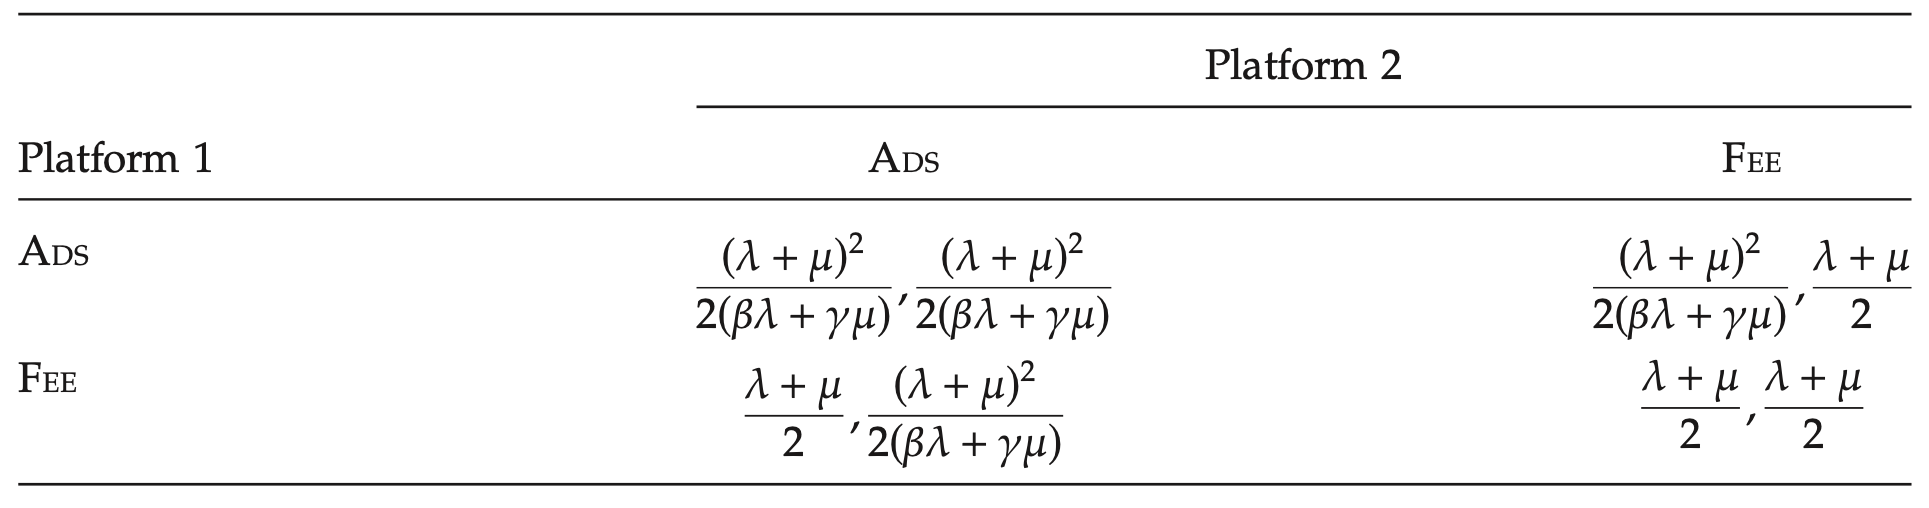
\includegraphics[width=\textwidth]{benchmark}
\end{frame}

\begin{frame}
    \frametitle{Benchmark}
    \framesubtitle{Payoff Matrix}
    \centering
    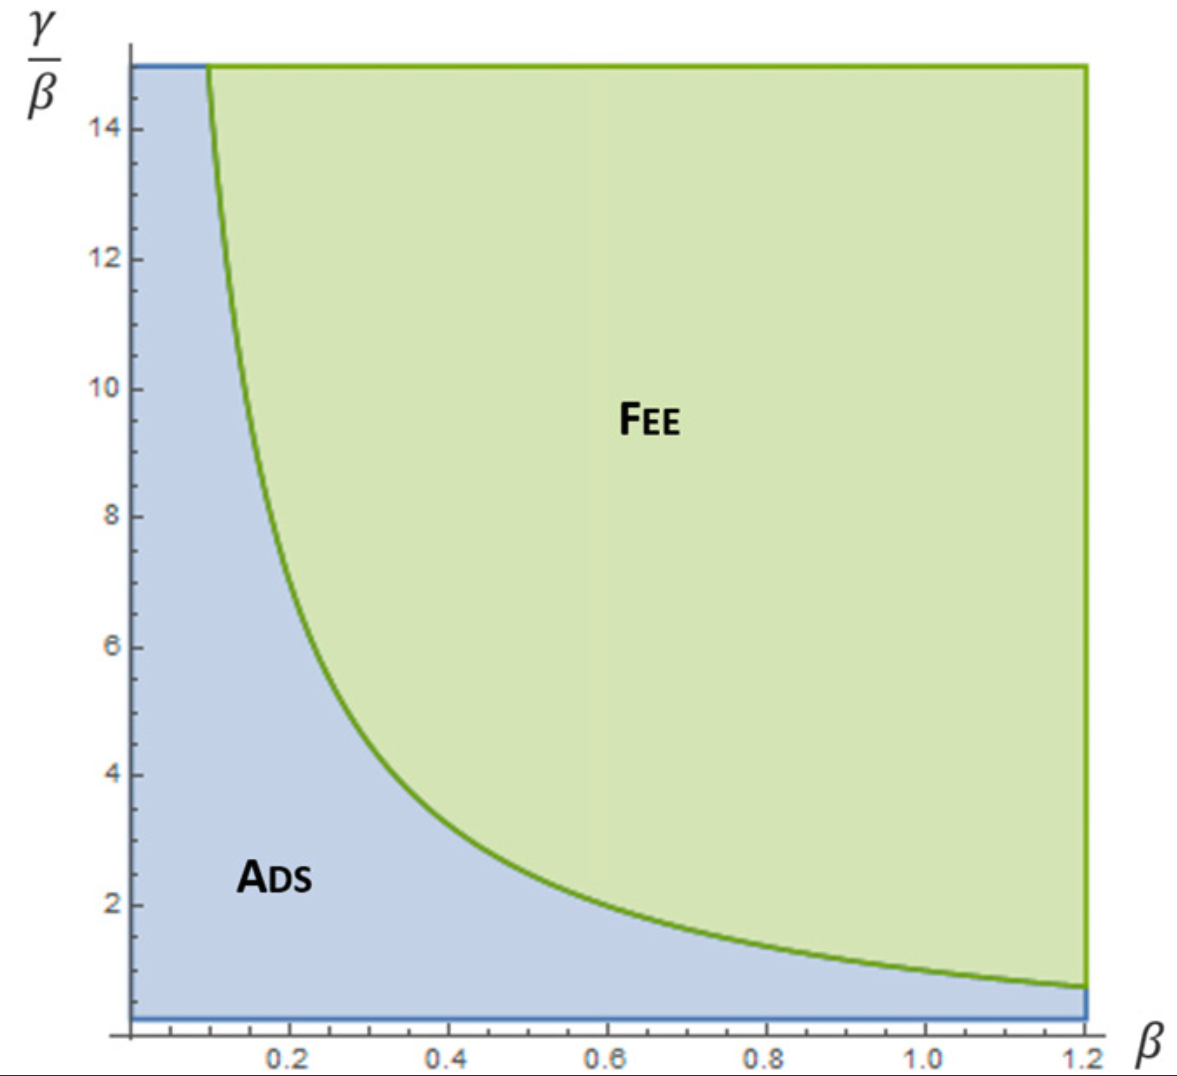
\includegraphics[width=0.6\textwidth]{benchfig}
\end{frame}


\section{Beneficial Ad Blockers}
\begin{frame}
    \frametitle{Platform Welfare}
    \begin{description}
        \item[Proposition 1:] 
            There is an equilibrium where \hl{both platforms allow ad blockers}. 
            In this equilibrium, when $\beta$ is sufficiently low and 
            $\frac{\gamma}{\beta}$ is sufficiently high, 
            platforms are better off than they would be if ad blockers did not exist.
        \item[Intuition:]
   \end{description}
            \begin{itemize}
                \item If platforms ban ad blockers, both segments of users see ads.
                However, due to the competition, platforms have no choice but to
                decrease the ad intensity $a_i$, which leads to low ad revenue.
                \item If platforms allow ad blockers, \hl{they do not need to compete the
                ad-block users} although they do not bring any revenue. However,
                they can \hl{discriminate users and raise the ad intensity $a_i$}
                to increase the profit.
            \end{itemize}
\end{frame}

\begin{frame}
    \frametitle{Platform Welfare}
    \framesubtitle{Intuition}
    \begin{itemize}
        \item Platforms want to be able to choose a different ad intensity 
            for segments of users with different ad sensitivity.
        \item However, this is an ideal. They cannot perfectly do that.
        \item \hl{Ad blockers provide an exogenous mechanism 
                to achieve a similar effect
            to help platforms discriminate users.}
        \item Ad-sensitive users self-select out of the market by using ad blockers.
    \end{itemize}
\end{frame}

\begin{frame}
    \frametitle{Platform Welfare}
    \framesubtitle{Summary}
    \begin{itemize}
        \item Platforms incentive to allow ad blockers
            \hl{as if the ad sensitivity of non-ad-block users $\beta$ is low
            and which of ad-block users $\gamma$ is high}.
        \item Three equilibria: $(\ban,\ban)$, $(\al,\al)$, and $(\fee,\fee)$.
        \item There are regions in the parameter space 
            with multi-equilibria,
            and we label better one in {\bf bold} in the following figure.
    \end{itemize}
    \centering
    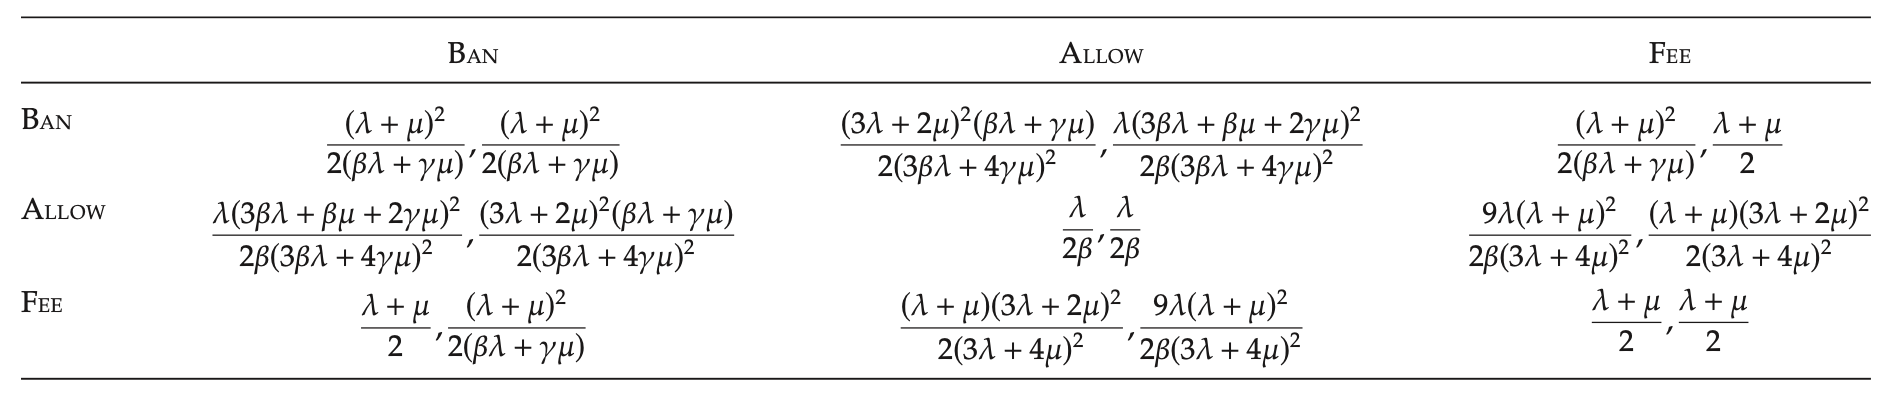
\includegraphics[width=0.95\textwidth]{platformpayoff}
\end{frame}

\begin{frame}
    \frametitle{Platform Welfare}
    \centering
    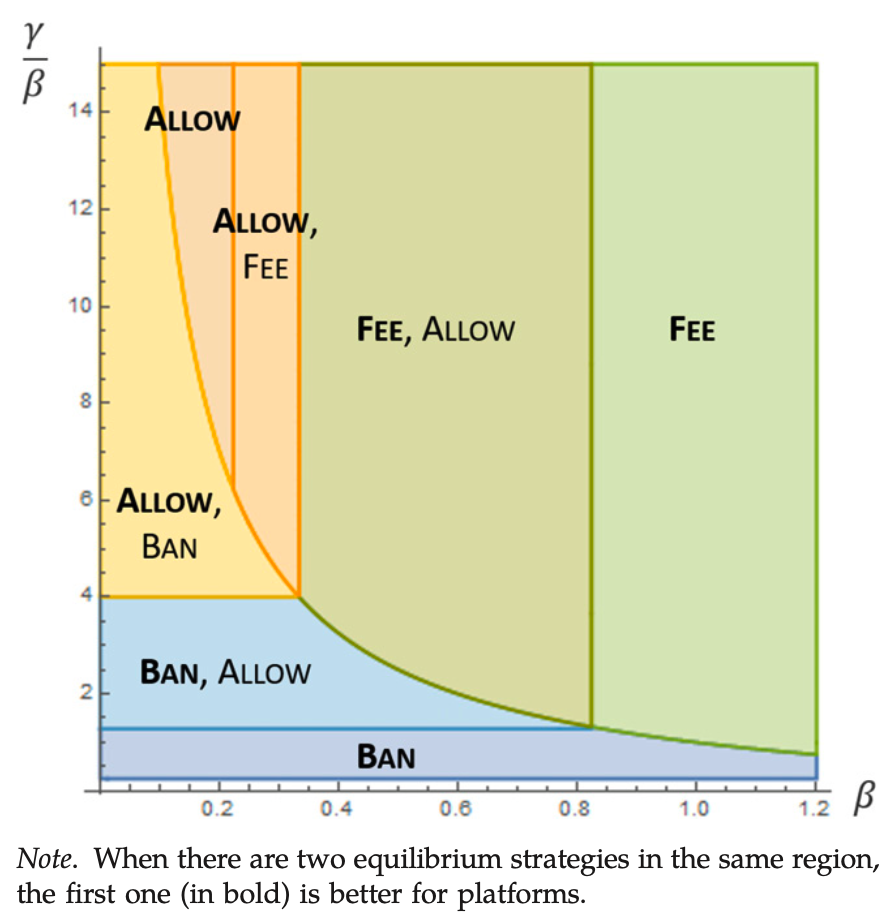
\includegraphics[width=0.6\textwidth]{platreg}
\end{frame}

\begin{frame}
    \frametitle{User Welfare}
    \begin{description}
        \item[Proposition 2:] Total user welfare is higher than 
            in the other two equilibria \hl{when both platforms allow ad blockers}.
            Moreover, some regions in the parameter space
            are better off by both users and 
            platforms.
        \item[Intuition:] Ad-block users get no disutility from ads because
            they block them, which improve the overall user utility even if
            non-ad-block users are sometimes worse off.
            \\
            \textcolor{myred}{My explanation:}
            as \nab are less sensitive, their disutilities
            affect lightly the overall user utility than \ab.
    \end{description}
\end{frame}

\begin{frame}%[label=current]
    \frametitle{Proof of Proposition 2}
    \framesubtitle{Optimal ad intensity in the \ban \ case}
    \begin{itemize}
        \item The indifferent \nab are at position $x_N$ satisfying
            $m+1-x_N-\beta a_1=m+x_N-\beta a_2 
            \iff x_N=\frac{1+\beta(a_2-a_1)}{2}$.
        \item The indifferent \ab are at position $x_A$ satisfying
            $m+1-x_A-\gamma a_1=m+x_A-\gamma a_2 
            \iff x_A=\frac{1+\gamma(a_2-a_1)}{2}$.
        \item The expected market share of platform 1 and 2
            is $(z_1,z_2)=(\lambda x_N+\mu x_A,\lambda (1-x_N)+\mu (1-x_A))$, 
            then the profit
            for both platforms is $(\Pi_1,\Pi_2)=(z_1a_1,z_2a_2)$.
        \item The optimal ad intensity $a_1$ and $a_2$ are derived by FOC, i.e.,
            $\frac{\partial\Pi_1}{\partial a_1}=\frac{\partial\Pi_2}{\partial a_2}=0$,
            which gives 
            \textcolor{myblue}{$a_1=a_2=\frac{\lambda+\mu}{\beta\lambda+\gamma\mu}$}.
    \end{itemize}
\end{frame}

\begin{frame}
    \frametitle{Proof of Proposition 2}
    \framesubtitle{User utility in the \ban \ case}
    \begin{itemize}
        \item Given ad intensity, the user utility when both platforms choose \ban \ is
            \small
            \setlength{\arraycolsep}{2.5pt}
            \medmuskip = 1mu
            \[
                \begin{array}{RL}
                    &u^\ban\\[3mm]
                    =&\lambda\left(\int_0^{\frac{1}{2}}\left(m+1-x-\beta\cdot
                        \frac{\lambda+\mu}{\beta\lambda+\gamma\mu}\right)dx 
                    +\int_{\frac{1}{2}}^1\left(m+x-\beta\cdot
                    \frac{\lambda+\mu}{\beta\lambda+\gamma\mu}\right)dx\right)\\[3mm]
                    +&\mu\left(\int_0^{\frac{1}{2}}\left(m+1-x-\gamma\cdot
                        \frac{\lambda+\mu}{\beta\lambda+\gamma\mu}\right)dx 
                    +\int_{\frac{1}{2}}^1\left(m+x-\gamma\cdot
                    \frac{\lambda+\mu}{\beta\lambda+\gamma\mu}\right)dx\right)\\[3mm]
                    =& (\lambda+\mu)\left(m-\frac{1}{4}\right).
                \end{array}
            \]
    \end{itemize}
\end{frame}

\begin{frame}
    \frametitle{Proof of Proposition 2}
    \framesubtitle{Optimal ad intensity in \al \ and \fee \ cases}
    \begin{itemize}
        \item Following the same steps above, we can derive the optimal
            ad intensity and the optimal subscription fee 
            when both platforms select \al \ and \fee, respectively.
        \item $a_1^\al=a_2^\al=\frac{1}{\beta}$ and $p_1=p_2=1$.
    \end{itemize}
\end{frame}

\begin{frame}
    \frametitle{Proof of Proposition 2}
    \framesubtitle{User utility in the \fee \ case}
    \begin{itemize}
         \item The user utility when both platforms choose \fee \ is
            \small
            \setlength{\arraycolsep}{2.5pt}
            \medmuskip = 1mu
            \[
                \begin{array}{RL}
                    & u^\fee \\[3mm]
                    =&\lambda\left(\int_0^{\frac{1}{2}}\left(m+1-x-1\right)dx 
                    +\int_{\frac{1}{2}}^1\left(m+x-1\right)dx\right)\\[3mm]
                    +&\mu\left(\int_0^{\frac{1}{2}}\left(m+1-x-1\right)dx 
                    +\int_{\frac{1}{2}}^1\left(m+x-1\right)dx\right)\\[3mm]
                    =& (\lambda+\mu)\left(m-\frac{1}{4}\right).
                \end{array}
            \]

    \end{itemize}
\end{frame}

\begin{frame}
    \frametitle{Proof of Proposition 2}
    \framesubtitle{User utility in the \al \ case}
    \begin{itemize}
        \item The user utility when both platforms choose \al \ is
            \small
            \setlength{\arraycolsep}{2.5pt}
            \medmuskip = 1mu
            \[
                \begin{array}{RL}
                    & u^\al \\[3mm]
                    =&\lambda\left(\int_0^{\frac{1}{2}}\left(m+1-x-\beta\cdot
                        \frac{1}{\beta}\right)dx 
                    +\int_{\frac{1}{2}}^1\left(m+x-\beta\cdot
                    \frac{1}{\beta}\right)dx\right)\\[3mm]
                    +&\mu\left(\int_0^{\frac{1}{2}}\left(m+1-x\right)dx 
                    +\int_{\frac{1}{2}}^1\left(m+x\right)dx\right)\\[3mm]
                    =& \lambda\left(m-\frac{1}{4}\right)+
                    \hl{\mu\left(m+\frac{3}{4}\right)}.
                \end{array}
            \]
        \item We can easily observe that
            $u^\al > u^\ban = u^\fee$.
    \end{itemize}
\end{frame}

\begin{frame}
    \frametitle{Benefits Summary}
    \begin{description}
        \item[Platforms:]
            Discriminate users with ad sensitivities and choose different
            ad intensity to maximize the profit.
        \item[Users:]
            Users can see ads by their willingness.

            Moreover, non-ad-block users are also better off since they obtain
            additional information, such as coupons, in ads.
            \begin{itemize}
                \item \hl{Everyone is strictly better off when allowing ad blockers.}
                \item People have an incentive to stop ad blockers after learning it
                    and obtain additional benefit.
            \end{itemize}
    \end{description}
\end{frame}

\section{Additional Strategies}
\begin{frame}
    \frametitle{New strategies}
    \begin{itemize}
        \item We investigate the effect of adding two strategies to
            the \hl{platforms}:
            \begin{description}
                \item[\aof:] Let users choose between watching ads
                    or paying for an ad-free plan.
                \item[\wl:] \hl{Pay a fee to the ad blocker 
                    to white-list their ads} among users employing the ad blocker.
            \end{description}
    \end{itemize}
\end{frame}

\begin{frame}
    \frametitle{\aof}
    \framesubtitle{}
    \begin{itemize}
        \item Instead of using ad blockers as a filter to discriminate users,
            platforms can also adopt \aof \ to segregate users by ad sensitivity.
        \item The \aof \ plan can be regarded as a combination of the \ban \
            and \fee \ plan, and it tries to achieve the best of both plans. 
        \begin{itemize}
            \item Ad-sensitive users will choose the fee option given this plan,
                which \hl{solves the problem in the \ban\ strategy} 
                that the ad-sensitive users force platforms to decrease ad intensity.
            \item Platforms are available to set a high ad intensity for \nab
                and charge a fee from \ab in the same time.
        \end{itemize}
    \end{itemize}
\end{frame}

\begin{frame}
    \frametitle{\aof}
    \framesubtitle{}
    \begin{itemize}
        \item \aof\ strategy seems to have the benefits of the \al\ strategy
            plus some extra fee revenue from \ab.
        \item However, does the \aof\ strategy always dominate the \al\ strategy?
            \begin{itemize}
                \item The answer, suprisingly, is \hl{not}.
            \end{itemize}
    \end{itemize}
    \begin{description}
        \item[Proposition 3:] There is still an equilibrium 
            where both platforms allow ad blockers even when adding the
            \aof\ plan. In addition,
            There are regions in the parameter space where this is the 
            unique equilibrium and regions where it is the best equilibrium 
            for platforms among others.
    \end{description}
\end{frame}

\begin{frame}
    \frametitle{\aof}
    \framesubtitle{}
    \begin{itemize}
        \item To derive the answer, we extend the model by considering the \aof\
            strategy.
            \begin{itemize}
                \item In this scenario, platforms need to decide two decision
                    variables: an \hl{ad intensity $a_i$} and a \hl{fee price $p_i$}.
            \end{itemize}
        \item We also refine the user ad sensitivity by adding a third segment of
            \nab\ in a mass $v$ and ad sensitivity $\eta$ to the model.
            \begin{itemize}
                \item The reason to do so is that the comparison of \aof\ and \al\
                    \hl{depends on the heterogeneity of the ad sensitivity for \nab}.
            \end{itemize}
    \end{itemize}
\end{frame}

\begin{frame}%[label=current]
    \frametitle{\aof}
    \framesubtitle{Intuition for Proposition 3}
    \begin{itemize}
        \item Now, we have three segment of users with different ad sensitivities.
            We may examine all possible sensitivities to measure two strategies.
        \item If $\gamma$ is very large compared with $\beta$ and $\eta$, platforms
            want to avoid showing ads to this segment as they will decrease the 
            ad intensity.
            \begin{itemize}
                \item Both \aof\ and \al\ strategies can achieve it.
            \end{itemize}
        \item If $\eta$ is sufficiently high, adopting the \aof\
            strategy is better for the platform since they avoid showing ads to 
            users with large ad sensitivity.
            \begin{itemize}
                \item \hl{What if $\eta$ starts decreasing toward $\beta$?}
            \end{itemize}
    \end{itemize}
\end{frame}

\begin{frame}%[label=current]
    \frametitle{\aof}
    \framesubtitle{Intuition for Proposition 3}
    \begin{itemize}
        \item \hl{As $\eta$ decreases}, the ad revenue from this segment \hl{increases}
            if they were forced to see ads.
        \item At some point, this revenue will exceed the revenue from the fee by
            this segment.
        \item Mathematically, it means $a>p$ but $\eta\cdot a<p$, which can happen
            when $\eta$ is sufficiently small.
            \begin{itemize}
                \item In this situation, platforms want these users to see ads but
                    they chooes the fee option when adopting \aof\ strategy, which
                    causes some loss of revenue.
                \item In the contrast, as there is no fee option in \al\ strategy,
                    such loss is covered.
            \end{itemize}
    \end{itemize}
\end{frame}

\begin{frame}%[label=current]
    \frametitle{When is \al\ better off?}
    \framesubtitle{}
    \begin{itemize}
        \item We already know that \al\ may be an equilibrium after considering \aof, 
            we want to describe when \al\ is the best strategy for platforms.
            \footnote{I use a symbol $\succ$ to represent the strategy preference. 
                $A\succ B$ indicates the strategy $A$ is better than $B$
            to platforms.}
    \end{itemize}
    \begin{description}
        \item[\al$\succ$\fee:] We want low $\beta$ and $\eta$ to increase ad intensity.
        \item[\al$\succ$\ban:] We want $\gamma>\beta$ and $\gamma>\eta$
            $\iff$ high $\frac{\gamma}{\beta}$ and $\frac{\gamma}{\eta}$.
        \item[\al$\succ$\aof:] We want $\eta\sim\beta$ closedly
            $\iff$ low $\frac{\eta}{\beta}$.
    \end{description}
    \begin{itemize}
        \item That is, for \al\ to be the best stategy, we want \hl{all subsegments of
            \nab to be nearly homogeneous in their sensitivities}, and \hl{be well
            separated from the \ab}.
    \end{itemize}
\end{frame}

\begin{frame}%[label=current]
    \frametitle{Payoff Matrix with \aof\ plan}
    \framesubtitle{}
    \centering
    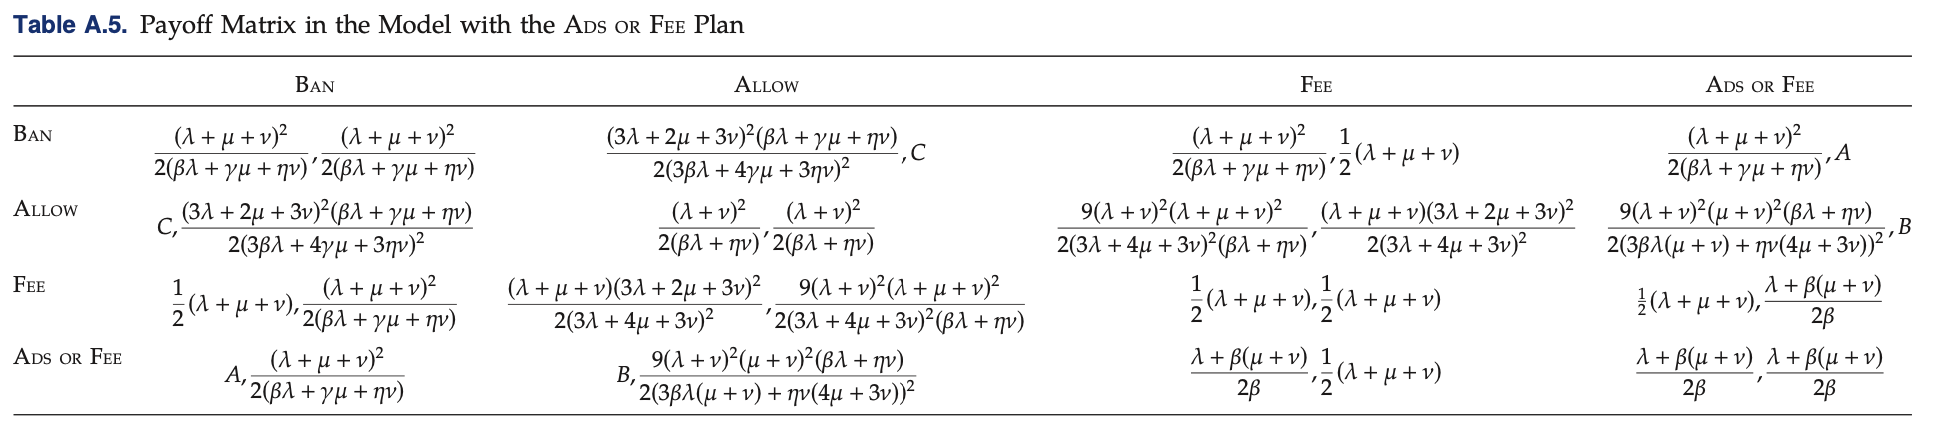
\includegraphics[width=1.05\textwidth]{aofpayoff}
\end{frame}

\begin{frame}%[label=current]
    \frametitle{Equilibrium Regions under Different Parameters}
    \framesubtitle{}
    \begin{figure}
        \centering
        \begin{subfigure}[b]{0.3\textwidth}
            \centering
            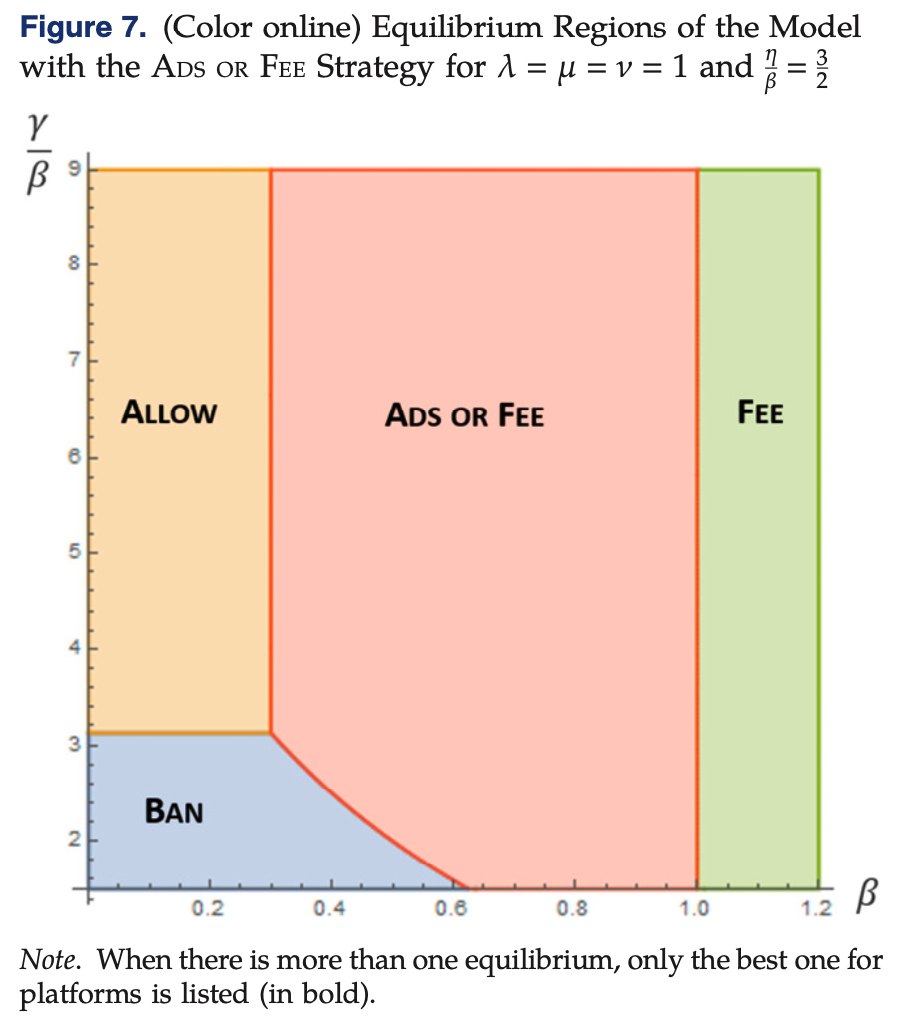
\includegraphics[width=\textwidth]{f7}
        \end{subfigure}
        \hfill
        \begin{subfigure}[b]{0.3\textwidth}
            \centering
            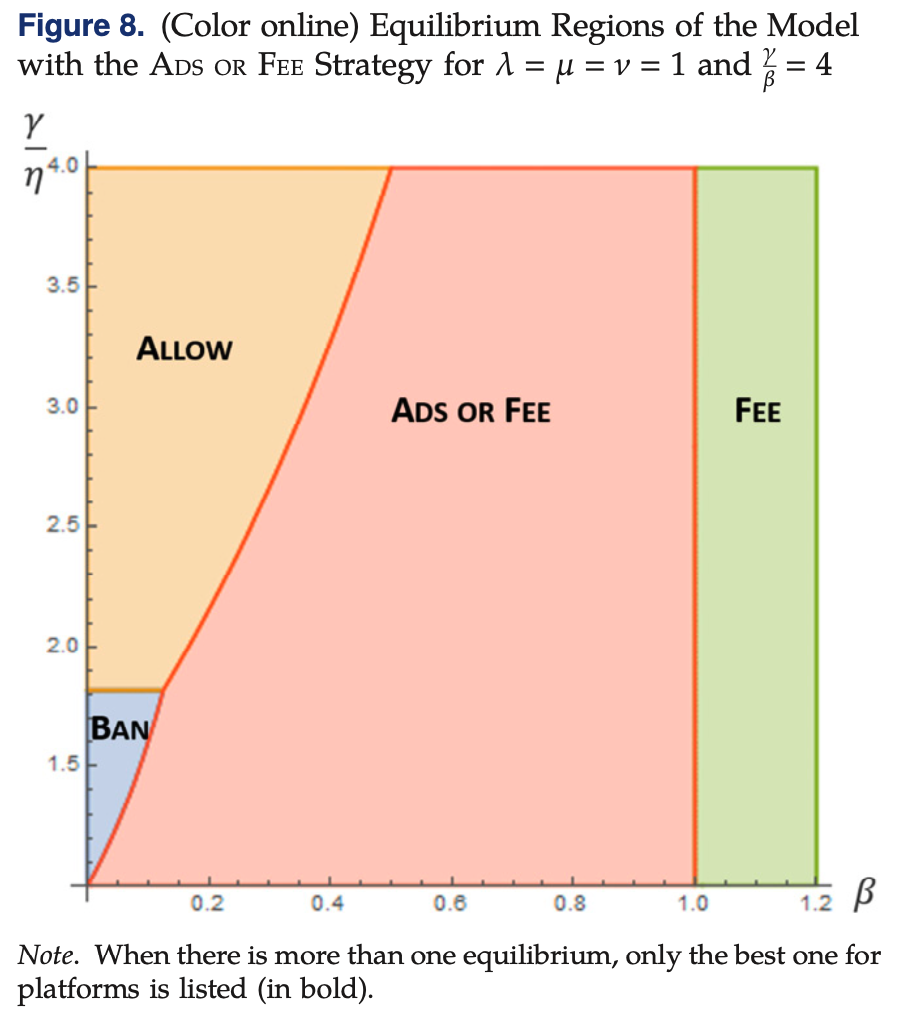
\includegraphics[width=\textwidth]{f8}
        \end{subfigure}
        \hfill
        \begin{subfigure}[b]{0.3\textwidth}
            \centering
            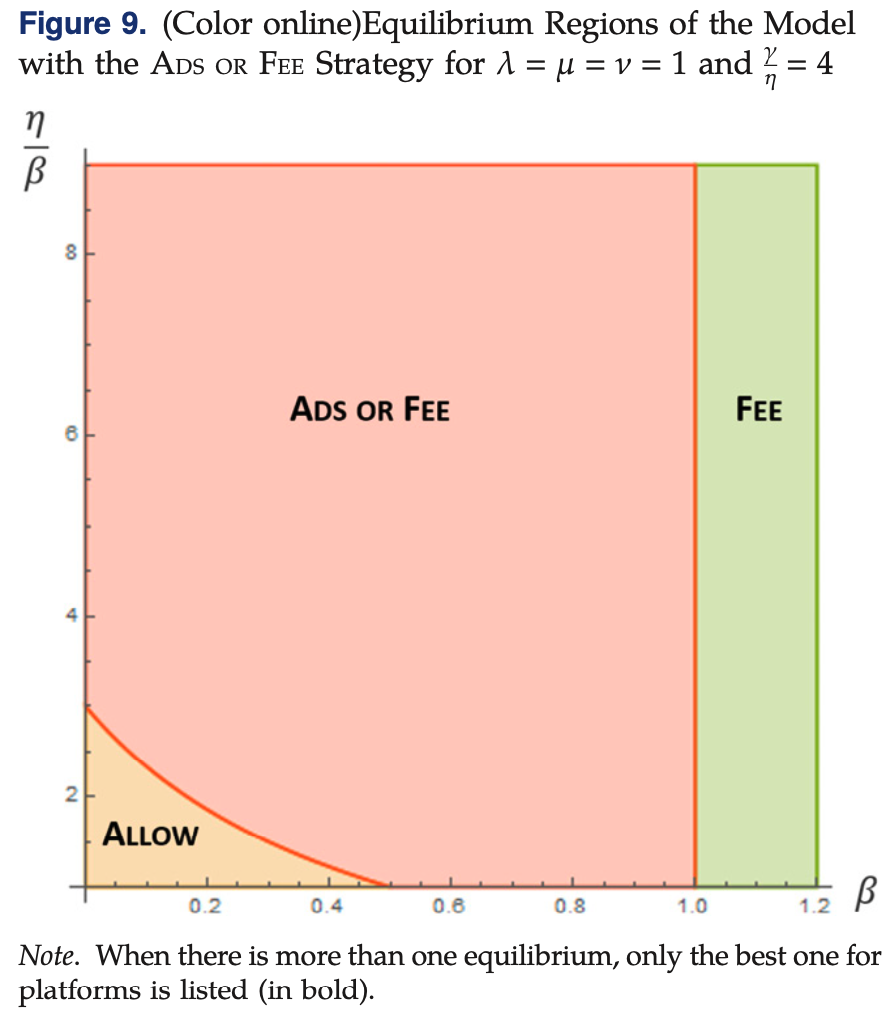
\includegraphics[width=\textwidth]{f9}
        \end{subfigure}
    \end{figure}
    \begin{itemize}
        \item Note that there may be still multi-equilibria in the regions,
            we only list the best one for platforms.
    \end{itemize}
\end{frame}

\begin{frame}%[label=current]
    \frametitle{Proof of Proposition 3}
    \framesubtitle{}
    \begin{itemize}
        \item The proof is similar to the case of the proof of Proposition 1
            but now with three segments of users and be more complicated.
        \item We illustrate only the case that both platforms use the \aof\ plan here to
            ease the note.
        \item Now we have \hl{four} strategies: \al, \ban, \fee, \aof, and \hl{three
            segments of users} separated from ad sensitivity: $\beta\leq\eta\leq\gamma$.
        \item This results in four subcases for platform 1:
            \[
                \begin{array}{LL}
                    \text{\textcolor{myblue}{$\triangleright$}}\;\;
                    p_1<\beta a_1\leq\eta a_1\leq\gamma a_1 &
                    \text{\textcolor{myblue}{$\triangleright$}}\;\;
                    \beta a_1\leq p_1\leq\eta a_1\leq\gamma a_1 \\
                    \text{\textcolor{myblue}{$\triangleright$}}\;\;
                    \beta a_1\leq\eta a_1<p_1\leq\gamma a_1 &
                    \text{\textcolor{myblue}{$\triangleright$}}\;\;
                    \beta a_1\leq\eta a_1\leq\gamma a_1<p_1.
                \end{array}
            \]
    \end{itemize}
\end{frame}

\begin{frame}%[label=current]
    \frametitle{Proof of Proposition 3}
    \framesubtitle{}
    \begin{itemize}
        \item Continue to analyze these four subcases but focus on the
            \textcolor{myred}{first} and the \textcolor{mygreen}{fourth} subcase:
            \[
                \begin{array}{LL}
                    \text{\textcolor{myred}{$\triangleright$}}\;\;
                    \text{\textcolor{myred}{$p_1<\beta a_1\leq\eta a_1\leq\gamma a_1$}} &
                    \text{\textcolor{myblue}{$\triangleright$}}\;\;
                    \beta a_1\leq p_1\leq\eta a_1\leq\gamma a_1 \\
                    \text{\textcolor{myblue}{$\triangleright$}}\;\;
                    \beta a_1\leq\eta a_1<p_1\leq\gamma a_1 &
                    \text{\textcolor{mygreen}{$\triangleright$}}\;\;
                    \text{\textcolor{mygreen}{$\beta a_1\leq\eta a_1\leq\gamma a_1<p_1$}}.
                \end{array}
            \]

        \item In the \textcolor{myred}{first} subcase, every user prefers to pay the fee,
            which is as if platform 1 chooses the \fee\ plan.
        \item In the \textcolor{mygreen}{fourth} subcase, it is as if platform 1 chooses the
            \ban\ plan.
        \item Therefore, \hl{we can ignore them}. This leaves us with two remaining subcases.
    \end{itemize}
\end{frame}

\begin{frame}%[label=current]
    \frametitle{Proof of Proposition 3}
    \framesubtitle{$\beta a_i\leq p_i\leq\eta a_i\leq\gamma a_i$}
    \begin{itemize}
        \item The first segment of indiffernet \nab are at position $x_N$ satisfying
            $m+1-x_N-\beta a_1=m+x_N-\beta a_2\iff x_N=\frac{1+\beta a_2-\beta a_1}{2}$.
        \item The second segment of indiffernet \nab are at position $x_{N,2}$ satisfying
            $m+1-x_{N,2}-p_1=m+x_{N,2}-p_2\iff x_{N,2}=\frac{1+p_2-p_1}{2}$.
        \item The indiffernet \ab are at position $x_A$ satisfying
            $m+1-x_{A}-p_1=m+x_{A}-p_2\iff x_A=\frac{1+p_2-p_1}{2}$.
   \end{itemize}
\end{frame}

\begin{frame}%[label=current]
    \frametitle{Proof of Proposition 3}
    \framesubtitle{$\beta a_i\leq p_i\leq\eta a_i\leq\gamma a_i$}
    \begin{itemize}
        \item The expected market shares of ads and fees of both platforms are
            $(z_{1,a},z_{2,a})=\left(\lambda x_N,\lambda(1-x_N)\right), \,
            (z_{1,p},z_{2,p})=\left(vx_{N,2}+\mu x_A, v(1-x_{N,2})+\mu(1-x_A)\right)$,
            and the profits are $(\Pi_1,\Pi_2)=(z_{1,a}a_1+z_{1,p}p_1,z_{2,a}a_2+z_{2,p}p_2)$.
        \item The optimal ad sensitivities and fees are derived by FOC, i.e.,
            $\frac{\partial\Pi_1}{\partial a_1}=\frac{\partial\Pi_1}{\partial p_1}=
            \frac{\partial\Pi_2}{\partial a_2}=\frac{\partial\Pi_2}{\partial a_2}=0$,
            which gives $a_1=a_2=\frac{1}{\beta}$ and $p_1=p_2=1$.
        \item We need to \hl{check the solution satisfying the inequality of this subcase}. Therefore,
            \hl{this subcase gives a possible equilibrium}.
        \item Following the same procedure, however, the solution to another subcase contradicts
            the inequality of it, hence, will not be a feasible equilibrium.
    \end{itemize}
\end{frame}

\subsection{\wl}
\begin{frame}%[label=current]
    \frametitle{\wl}
    \framesubtitle{}
    \begin{itemize}
        \item Another plan is to ask the ad blockers to \wl\ platforms' ads.
        \item This idea was launched from Adblock Plus, the most popular ad-blocker.
            Big techs pays monthly fee to participate in this program to avoid their 
            ads being blocked.
        \item Moreover, Adblock Plus also started selling "accepable" ads to publishers.
        \item This policy was criticized by lots of businessmen, including
            pulishers and advertisers; they regard it as
            extorted, unethical and immoral.
            \begin{itemize}
                \item They now have to share part of reveue with it.
            \end{itemize}
        \item However, \wl\ services are also the main source of revenue for Adblock Plus.
        \item The key question is: \hl{whether adopting this new option benefits platforms?}
    \end{itemize}
\end{frame}

\begin{frame}%[label=current]
    \frametitle{\wl}
    \framesubtitle{}
    \begin{itemize}
        \item To answer this question, we extend the original model.
            \begin{itemize}
                \item Enable \wl\ strategy to platforms: \al, \ban, \fee, and \wl\ in this discussion.
                \item Platforms pay $f\geq0$ to ad-blocker company to display their ads if choosing
                    this strategy. Note that in this context, platforms still allow
                    ad blockers.
                \item Three users segments: \\ one of \hl{\nab} 
                    of mass $\lambda$ and ad sensitivity $\beta$;
                    \\ one of \ab \hl{feel ok with \wl\ policy} of mass $\xi$ and ad sensitivity $\zeta$;
                    \\ one of \ab \hl{are against all ads} of mass $\mu$ and ad sensitivity $\gamma$.
                \item \hl{No any assumption imposed on relationship between $\beta$,$\xi$, and $\gamma$.}
            \end{itemize}
    \end{itemize}
\end{frame}

\begin{frame}%[label=current]
    \frametitle{\wl}
    \framesubtitle{Proposition and intuition}
    \begin{description}
        \item[Proposition 4:] When allowing \wl\ strategy, both platforms select \wl\ is an equilibrium. 
            In this equilibrium, platforms are sometimes better of than the benchmark.
        \item[Intuition:] Remind the context of three segments. Consider the case that 
            $\beta\leq\zeta\leq\gamma$, that is, \hl{the users' behavior reveal their preference of ad
            sensitivity.} Therefore, the \wl\ option can help platforms \hl{separate the two type
            of \ab.}
    \end{description}
\end{frame}

\begin{frame}%[label=current]
    \frametitle{When is \wl\ better off?}
    \framesubtitle{}
    \begin{itemize}
        \item We want to find the condition where \wl\ is the best option.
            \footnote{I use a symbol $\succ$ to represent the strategy preference. 
            $A\succ B$ indicates the strategy A is better than B to platforms.}
    \end{itemize}
    \begin{description}
        \item[Small $f$:] First, we need a sufficiently small $f$ or it will be lavish.
        \item[\wl$\succ$\fee:] We want low $\beta$ and $\zeta$ to increase ad intensity.
        \item[\wl$\succ$\ban:] We want $\gamma>\beta$ and $\gamma>\zeta\iff$ high
            $\frac{\gamma}{\beta}$ and $\frac{\gamma}{\zeta}$.
        \item[\wl$\succ$\al:] We want $\zeta\sim\beta$ closedly $\iff$ low $\frac{\zeta}{\beta}$.
    \end{description}
    \begin{itemize}
        \item That is, for \wl\ to be the best strategy, we want two sub-segments of \ab to be
            heterogeneous and well separated, and low ad sensitivity of \nab.
    \end{itemize}
\end{frame}

\begin{frame}%[label=current]
    \frametitle{Payoff Matrix with \wl\ Plan}
    \framesubtitle{}
    \centering
    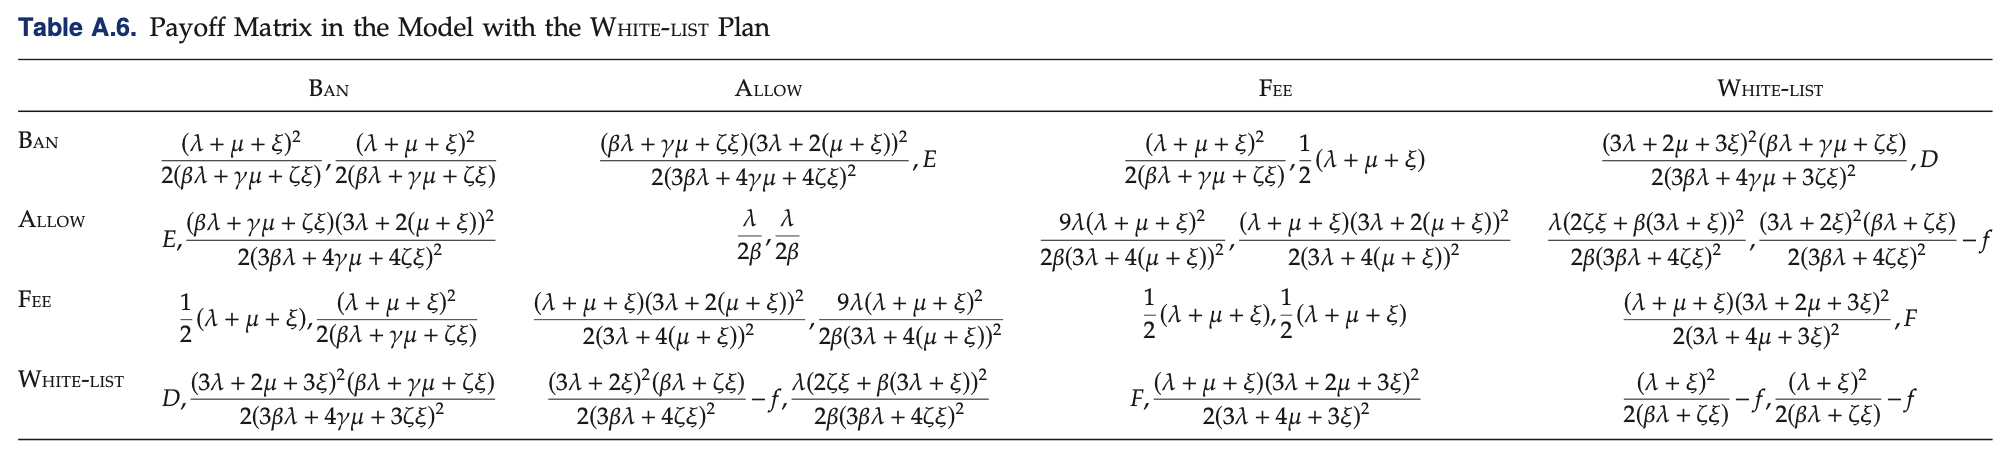
\includegraphics[width=\textwidth]{wlrev}
\end{frame}

\begin{frame}%[label=current]
    \frametitle{Equilibrium Regions under Different Parameters}
    \framesubtitle{}
    \begin{figure}
        \centering
        \begin{subfigure}[b]{0.3\textwidth}
            \centering
            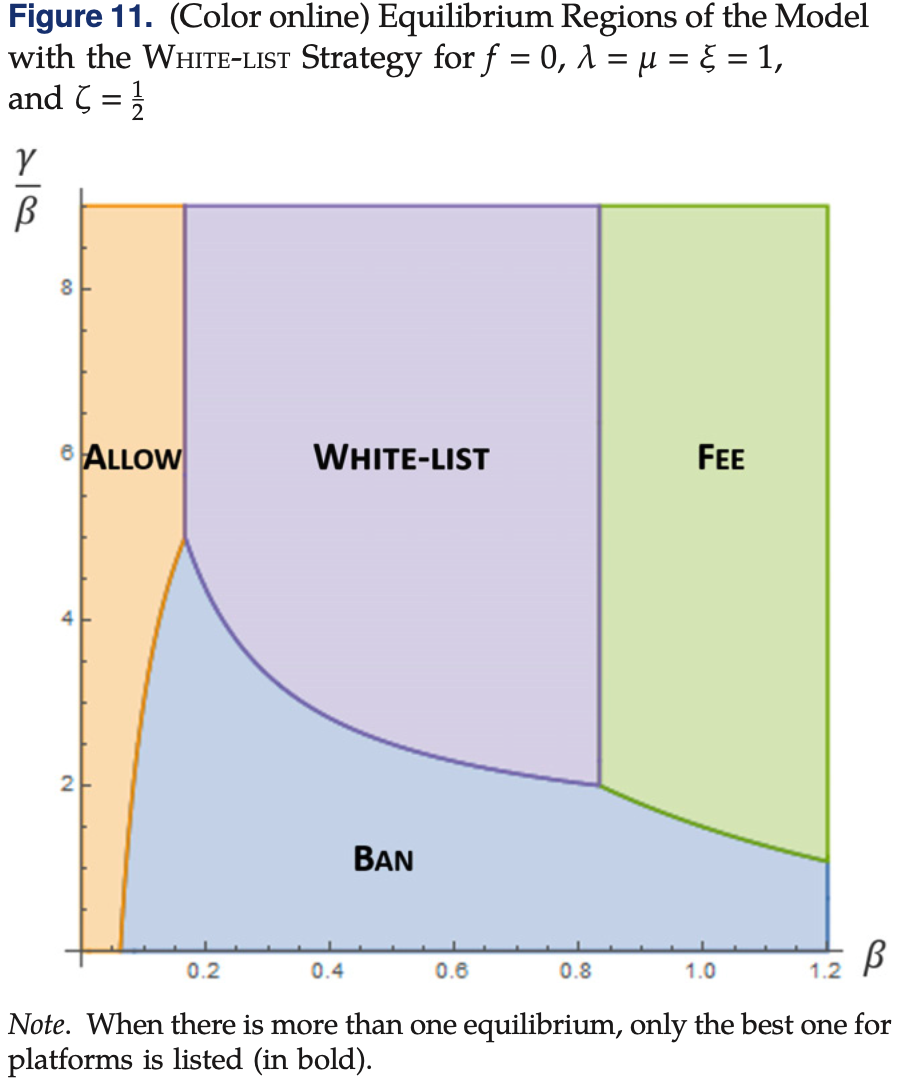
\includegraphics[width=\textwidth]{f11}
        \end{subfigure}
        \hfill
        \begin{subfigure}[b]{0.3\textwidth}
            \centering
            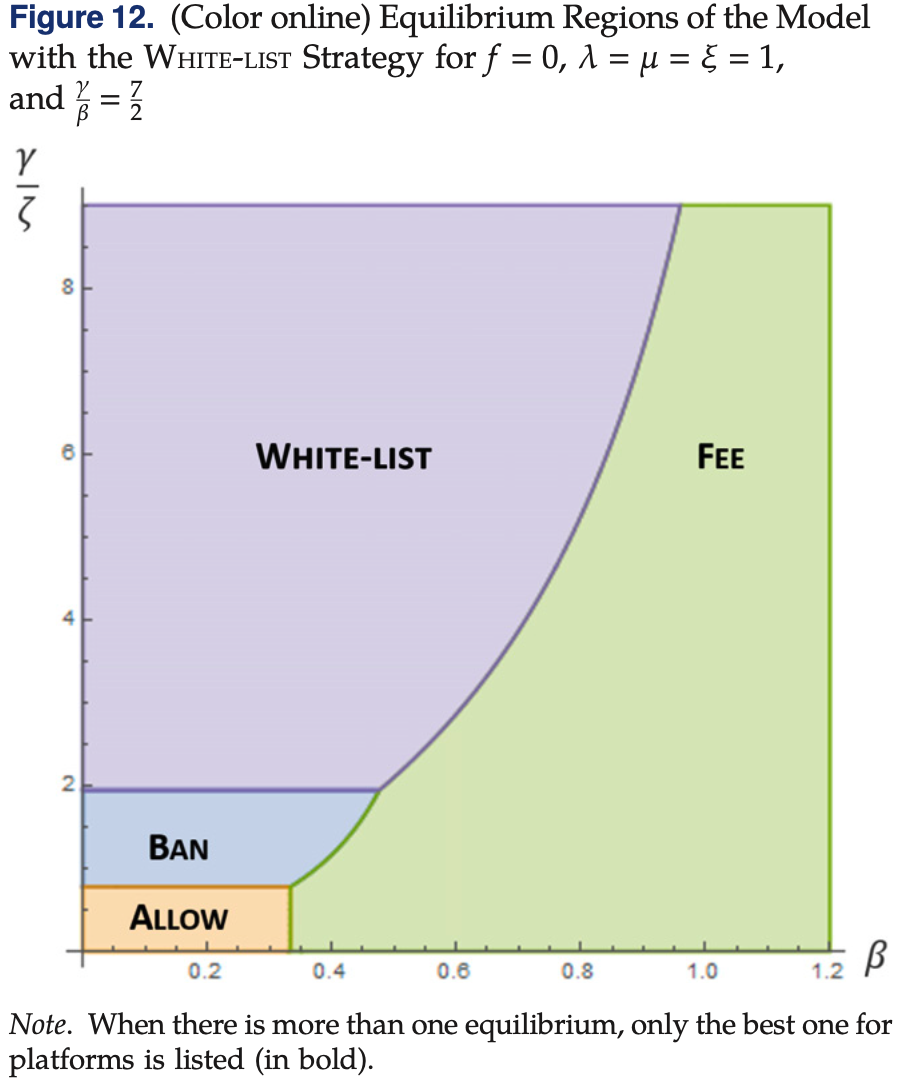
\includegraphics[width=\textwidth]{f12}
        \end{subfigure}
        \hfill
        \begin{subfigure}[b]{0.3\textwidth}
            \centering
            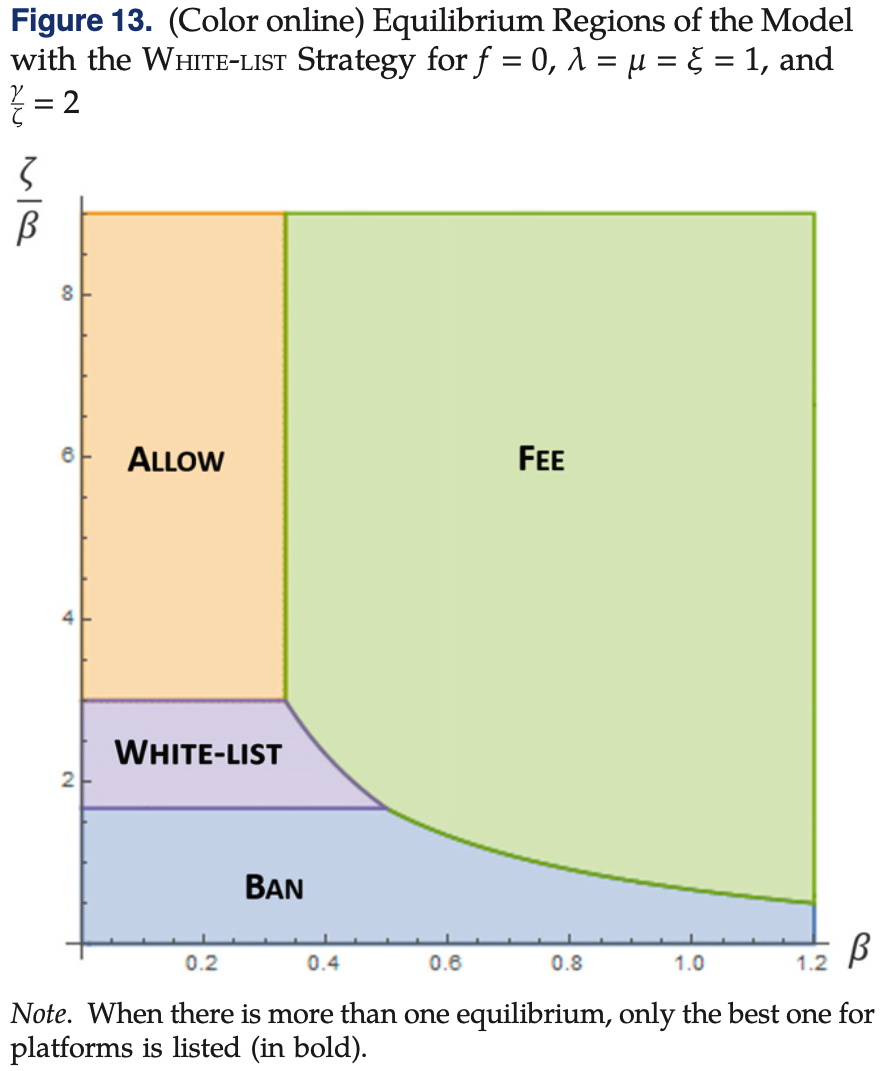
\includegraphics[width=\textwidth]{f13}
        \end{subfigure}
    \end{figure}
    \begin{itemize}
        \item Note that there may be still multi-equilibria in the regions,
            we only list the best one for platforms.
    \end{itemize}
\end{frame}



\section{Quality of Content}
\begin{frame}%[label=current]
    \frametitle{Quality of Content}
    \framesubtitle{}
    \begin{itemize}
        \item The quality of content affects users' decision of which platform to join.
        \item User Generated Content (UGC) and Professionally Generated Content (PGC) are two
            main content sources of platforms.
        \item The revenue-sharing model differs between UGC and PGC. In UGC, platforms
            with the subscription policy share their revenue with content creators.
            \begin{itemize}
                \item For example, YouTube shares $55\%$ revenues from ads and subscriptions with
                    creators.
            \end{itemize}
        \item The question is: how the quality of content is affected by the advent of ad blockers
            under a revenue-sharing model with the subscriptions policy.
    \end{itemize}
\end{frame}

\begin{frame}%[label=current]
    \frametitle{Model extension}
    \begin{itemize}
        \item To answer this question, we extend the model by \hl{adding content creators}.
        \item Assume that two platforms have their own content creators. Content creators
            have to \hl{decide the quality of content $q_i$}, and they \hl{incur some cost
            $c_i\cdot q_i^2$} when generating content with quality $q_i$.
        \item We include an additional term $r\cdot q_i$ to user's utility to capture the effect
            of quality of content.
        \item Each platform \hl{decides a fixed fraction $f_i$ 
            to share the revenue with their content creators}.
    \end{itemize}
\end{frame}

\begin{frame}%[label=current]
    \frametitle{Model extension}
    \begin{itemize}
        \item The profits for \cc in platform $i$ and platform are
            \[
                \begin{array}{L}
                    \Pi_i^\text{Content Creators}
                    =f_i\cdot(\text{Total revenue for platform $i$})-c_iq_i^2 \\[3mm]
                    \Pi_i^\text{Platform}=(1-f_i)(\text{Total revenue for platform $i$}).
                \end{array}
            \]
        \item The game proceeds the same as before with the addition:
            The platform and \cc determine determine the strategy and the quality of content
            in the first step, respectively, then users choose between the platforms in the second step.
    \end{itemize}
\end{frame}

\begin{frame}%[label=current]
    \frametitle{Proposition and Intuition}
    \begin{description}
        \item[Proposition 5:] All the results of the basic model are robust under this extension.
            In addition, the quality of content is higher for sufficiently high $\frac{\gamma}{\beta}$
            and sufficiently low $\beta$.
            Moreover, there is an equilibrium that platforms, users, and \cc are better off.
        \item[Intuition:] If the platform adopts the \ban\ or \fee\ strategies, all the extra value
            generated by the quality of content are collected by the platform and \cc.
            However, if the platform allows ad blockers, extra value from the higher quality of content
            benefits users.
    \end{description}
\end{frame}

\section{Assumption Relaxation}
\begin{frame}%[label=current]
    \frametitle{Assumption Relaxation}
    \begin{itemize}
        \item Remind that we impose two simplifying assumptions to the model:
            \begin{itemize}
                \item Users without an ad blocker always suffer a negative linear
                    utility from advertising.
                \item Users with an ad blocker are only those with high ad sensitivity.
            \end{itemize}
        \item We want to examine the necessity of these two assumptions.
    \end{itemize}
\end{frame}

\begin{frame}%[label=current]
    \frametitle{First Assumption}
    \framesubtitle{Concave Utility from Ads}
    \begin{itemize}
        \item To remove the first assumption, we assume that the consumers' utility function
            to ads is \hl{concave}.
            \begin{itemize}
                \item It is reasonable because ads in low quantities can actually benefit users
                    for getting extra information.
                \item However, on the other hand, ads in high quantities become annoying and
                    result in a negative utility for consumers.
            \end{itemize}
    \end{itemize}
\end{frame}

\begin{frame}%[label=current]
    \frametitle{Second Assumption}
    \framesubtitle{Endogenous Decisions}
    \begin{itemize}
        \item To remove the second assumption, we assume that 
            \hl{all users can use ad blockers whenever they want}, depending on their utility.
        \item Users still have varying ad sensitivity, which is expressed by their utility function:
            \[
                \begin{array}{L}
                    u_L(a_i)= \begin{cases}
                        \delta a_i & \text{if } a_i\leq a^* \\
                        \delta a^* + L(a^*-a_i) & \text{otherwise}
                    \end{cases} \\
                    u_H(a_i)= \begin{cases}
                        \delta a_i & \text{if } a_i\leq a^* \\
                        \delta a^* + H(a^*-a_i) & \text{otherwise,}
                    \end{cases}
                \end{array}
            \]
            where $H\geq L\geq0$ and $\delta,a^*\geq0$.
    \end{itemize}
\end{frame}

\begin{frame}%[label=current]
    \frametitle{Proposition and Intuition}
    \framesubtitle{}
    \begin{description}
        \item[Proposition 6:] When users have a concave utility from ads
            and their decision to use an ad blocker or not is endogenous, 
            there is an equilibrium where both platforms allow ad blockers. 
            In this equilibrium, when $L$ is sufficiently low and 
            $\frac{H}{L}$ is sufficiently high,
            platforms are better off.
        \item[Intuition:] 
            The competition between platforms will decrease ad intensity if both platforms
            adopts \ban\ strategy, which decline the revenue. If using \al\ strategy,
            platforms can avoid competing high ad-sensitive users and increase the 
            ad intensity for those seeing ads.
    \end{description}
\end{frame}

\section{Conclusion}
\begin{frame}[label=current]
    \frametitle{Managerial Implications}
    \begin{itemize}
        \item This research can provide websites with general guidelines regarding the plan
            they should choose based on the heterogeneity of ad sensitivity for their visitors.
    \end{itemize}
    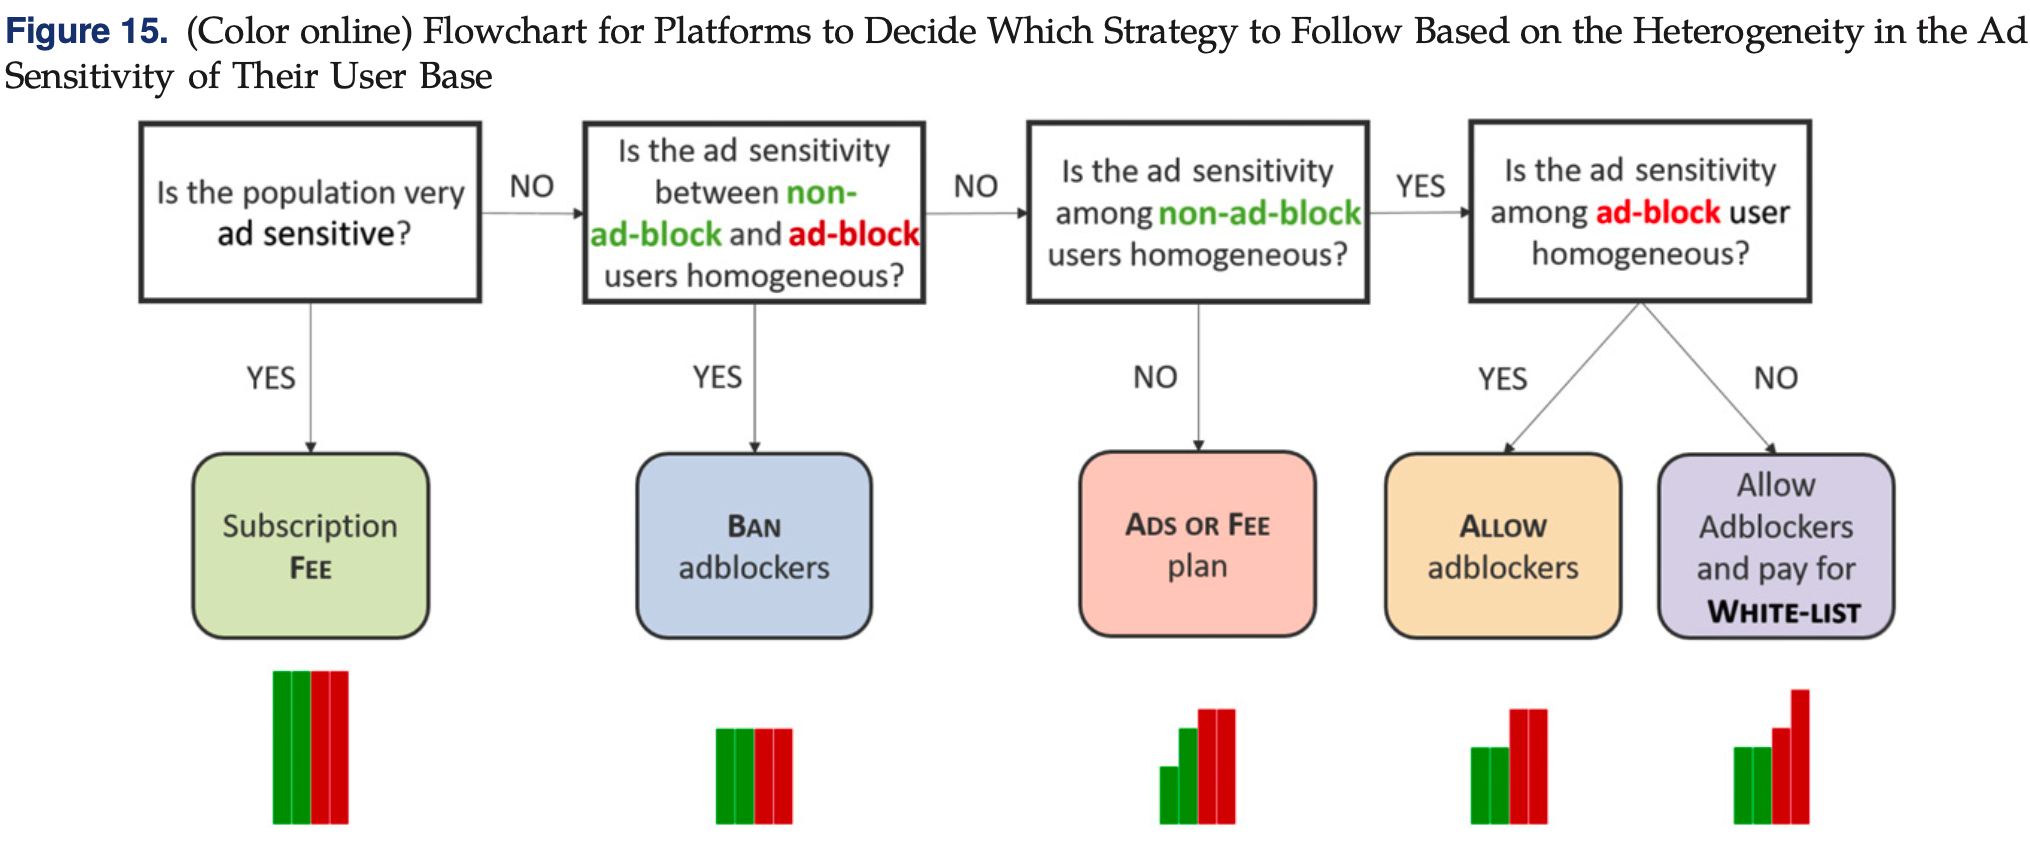
\includegraphics[width=\textwidth]{flow}
\end{frame}

\begin{frame}[allowframebreaks]
    \bibliography{ref}
\end{frame}

%\end{CJK*}
\end{document}

